\documentclass[UTF8,zihao=-4]{ctexart}
\usepackage[a4paper,margin=2.5cm]{geometry}
\usepackage{amsmath, amssymb, amsthm}
\usepackage{bm}
\usepackage{hyperref}
\usepackage{graphicx}
\usepackage{caption}
\usepackage{listings}
\usepackage{xcolor}
\usepackage{float}
\usepackage{placeins}
\graphicspath{{figures/}}

% Code style
\lstdefinestyle{code}{
  basicstyle=\ttfamily\small,
  numbers=left,
  numberstyle=\tiny,
  numbersep=8pt,
  keywordstyle=\color{blue},
  commentstyle=\color{teal!70!black},
  stringstyle=\color{orange!70!black},
  showstringspaces=false,
  breaklines=true,
  frame=single,
  framerule=0.3pt,
  rulecolor=\color{black!15}
}
\lstset{style=code}

\title{卷积神经网络详解}
\author{}
\date{\today}

\begin{document}
\maketitle

\section{CNN 结构与工作原理}
卷积神经网络(CNN)利用局部连接、权值共享与平移不变性来处理图像等空间结构数据。输入张量 $\mathbf{X} \in \mathbb{R}^{C_{\text{in}} \times H \times W}$ 与卷积核 $\mathbf{K} \in \mathbb{R}^{C_{\text{out}} \times C_{\text{in}} \times k_h \times k_w}$ 通过
\begin{equation}
  Y_{c,i,j} = \sum_{c'=1}^{C_{\text{in}}} \sum_{u=0}^{k_h-1} \sum_{v=0}^{k_w-1} K_{c,c',u,v} \, X_{c',\, i s + u - p,\, j s + v - p}
\end{equation}
得到特征图,其中 $s$ 为步幅、$p$ 为填充。步幅决定下采样倍率,padding 用于保留边界信息。图~\ref{fig:cnn_structure_cn} 展示了多层卷积如何逐渐扩大感受野。

\subsection{层级特征表示}
浅层卷积通常学习边缘、纹理等低级特征;中层捕捉局部组合结构;更深层可编码对象语义。共享权重显著减少参数量,使 CNN 在硬件有限的情况下也能训练。

\subsection{填充、步幅与膨胀卷积}
零填充或反射填充可在计算时覆盖边界像素。膨胀(空洞)卷积通过在核元素间插入间隔扩大神经元感受野,其有效核大小为 $(k-1)d+1$。合理搭配步幅与膨胀率可在保持分辨率的同时引入全局上下文。

\subsection{池化与下采样}
池化层对局部区域求最大值或平均值,增强平移鲁棒性。也可以用带步幅的卷积取代固定池化,使下采样过程可以学习。全局平均池化将每个通道压缩成单个数值,常用于分类头部。

\subsection{归一化与激活函数}
ReLU 及其变体(LeakyReLU、GELU)提供非线性能力。BatchNorm 使用批统计量归一化激活,缓解内部协变量偏移并允许更大学习率;当批量较小时,可采用 LayerNorm 或 GroupNorm。组合合适的归一化与激活对深层 CNN 至关重要。

\begin{lstlisting}[language=Python, caption={带归一化与池化的 PyTorch 卷积 stem 模块。}]
import torch.nn as nn

class ConvStem(nn.Module):
    def __init__(self, in_channels=3, hidden_channels=(64, 128, 256)):
        super().__init__()
        layers = []
        current = in_channels
        for out_channels in hidden_channels:
            layers += [
                nn.Conv2d(current, out_channels, kernel_size=3, stride=1, padding=1, bias=False),
                nn.BatchNorm2d(out_channels),
                nn.ReLU(inplace=True),
                nn.MaxPool2d(kernel_size=2, stride=2)
            ]
            current = out_channels
        self.stem = nn.Sequential(*layers)

    def forward(self, x):
        return self.stem(x)
\end{lstlisting}

\begin{figure}[H]
  \centering
  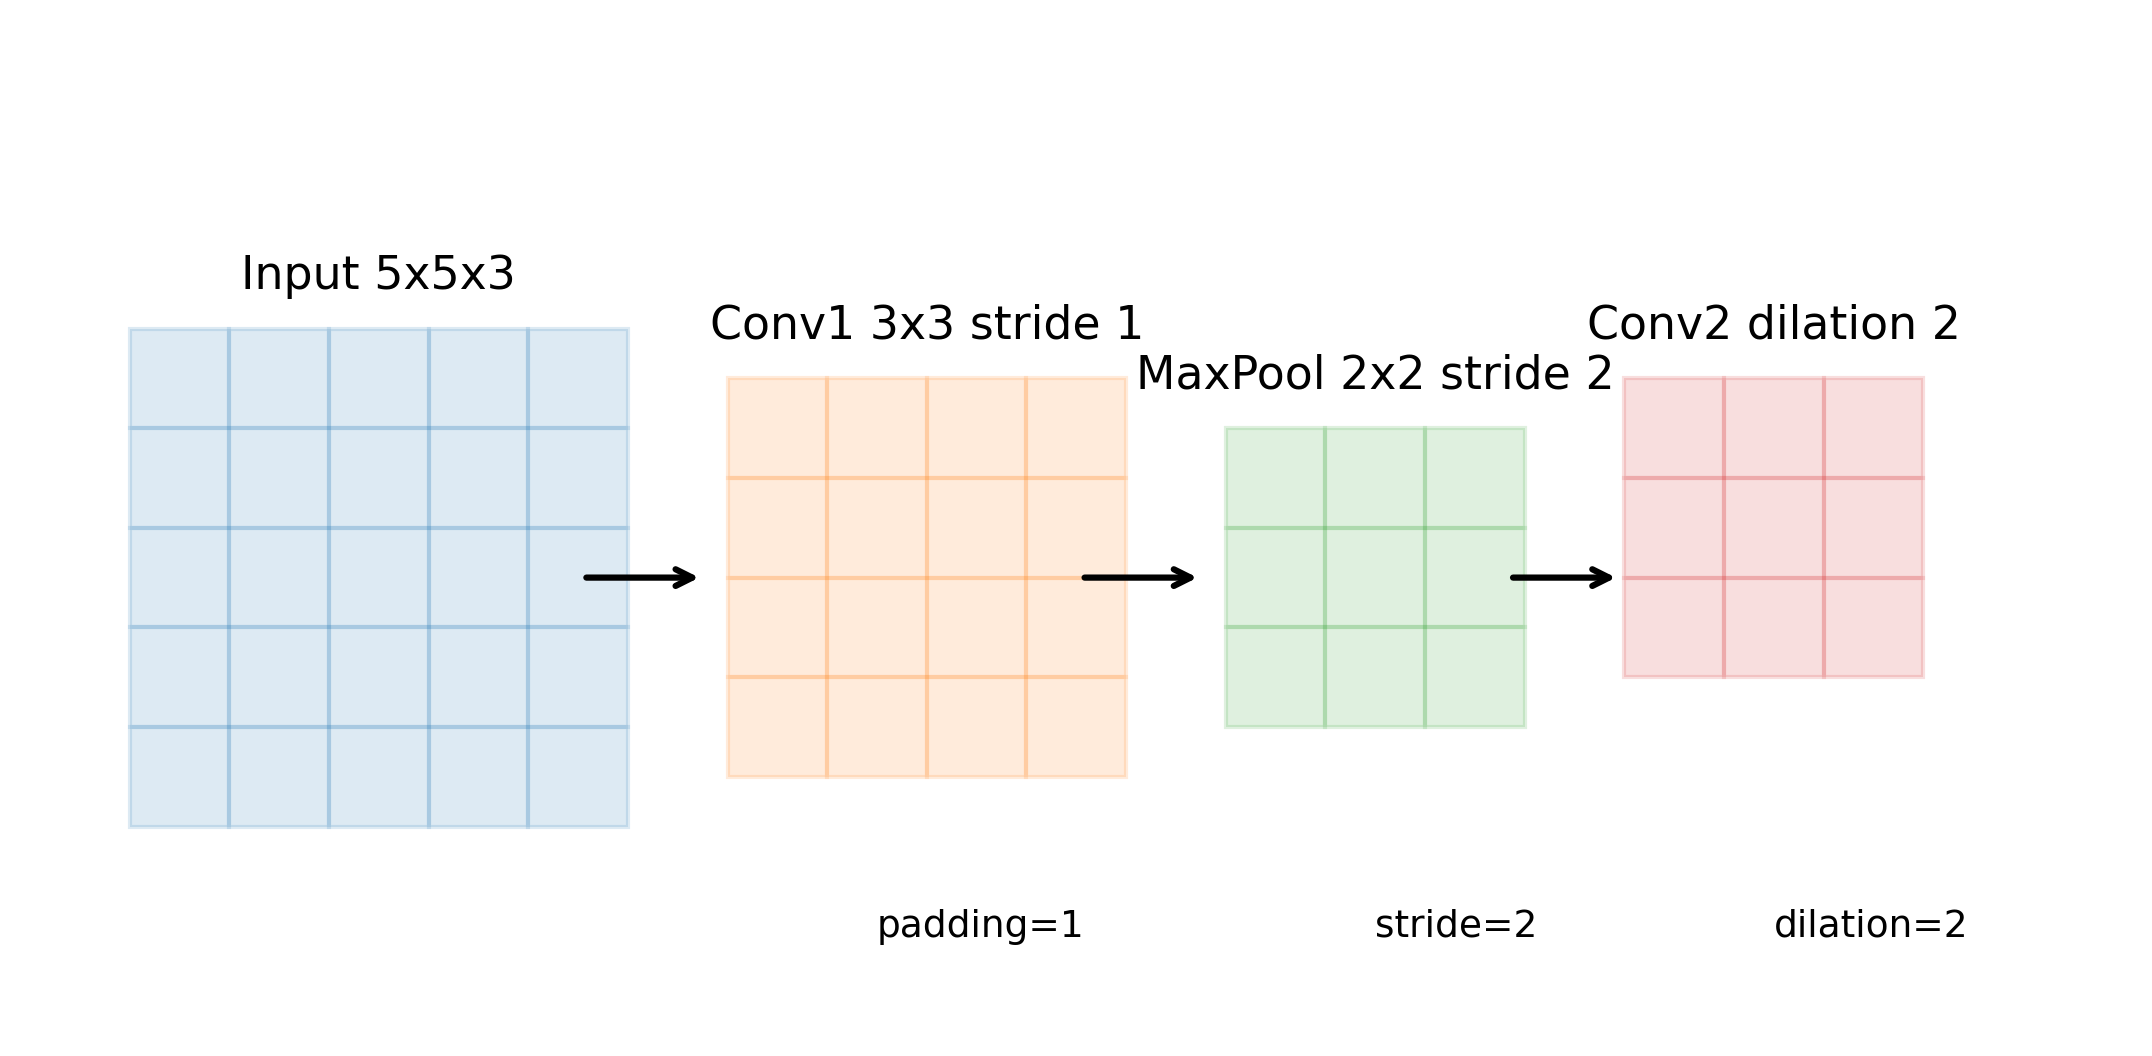
\includegraphics[width=0.85\linewidth]{cnn_structure_receptive_field.png}
  \caption{卷积、padding、步幅与池化在多层网络中扩展感受野的示意图。}
  \label{fig:cnn_structure_cn}
\end{figure}
\FloatBarrier

\section{经典网络对比:LeNet 至 EfficientNet}
自 1990 年代以来,CNN 架构不断演进以解决优化难题、提升效率并兼顾可扩展性。图~\ref{fig:cnn_timeline_cn} 总结了关键里程碑,表~\ref{tab:cnn_compare_cn} 对比了代表模型的深度、参数量与核心思想。

\subsection{LeNet-5(1998)}
LeNet 通过卷积 + 子采样 + 全连接结构实现手写数字识别,被视为现代 CNN 的雏形。其权值共享思想显著减轻了参数规模。

\subsection{AlexNet(2012)}
AlexNet 在 ImageNet 大赛上力压传统方法,关键创新包括 ReLU 激活避免饱和、使用 GPU 训练、重度数据增强与 dropout 正则化。

\subsection{VGG(2014)}
VGG-16/19 采用统一的 $3\times3$ 小卷积堆叠成深层网络,展示了深度与小卷积核的强大组合。结构简单,易于迁移到其他任务。

\subsection{ResNet(2015)}
ResNet 引入残差连接,将目标函数表示为 $\mathcal{F}(\mathbf{x}) + \mathbf{x}$,有效缓解梯度消失,并可训练 100 层以上网络。瓶颈模块用 $1\times1$ 卷积压缩通道以提升效率。

\subsection{Inception 系列(2014--2016)}
GoogLeNet 使用多分支模块同时捕捉不同尺度特征,并结合 $1\times1$ 卷积降维。后续版本增加了模块因式分解、批归一化与正则化手段,显著提升精度与效率。

\subsection{EfficientNet(2019)}
EfficientNet 以复合缩放系数统一调整网络深度、宽度与输入分辨率;核心使用带 Squeeze-and-Excitation 注意力的 MBConv 模块,在有限 FLOPs 下达到高准确率。

\begin{table}[H]
  \centering
  \caption{经典 CNN 架构对比(ImageNet 规模,参数与 FLOPs 为近似值)。}
  \label{tab:cnn_compare_cn}
  \begin{tabular}{lccccl}
    \hline
    架构 & 年份 & 层数 & 参数量 (M) & FLOPs (G) & 核心亮点 \\
    \hline
    LeNet-5 & 1998 & 7 & 0.06 & 0.002 & 卷积 + 子采样\shortrule\
    AlexNet & 2012 & 8 & 61 & 1.5 & ReLU、dropout、大卷积核 \\
    VGG-16 & 2014 & 16 & 138 & 15.5 & 堆叠 $3\times3$ 小核 \\
    ResNet-50 & 2015 & 50 & 25 & 4.1 & 残差瓶颈块 \\
    Inception-v3 & 2016 & 48 & 24 & 5.7 & 多分支 + 因式分解卷积 \\
    EfficientNet-B4 & 2019 & 82 & 19 & 4.2 & 复合缩放、MBConv \\
    \hline
  \end{tabular}
\end{table}

\begin{figure}[H]
  \centering
  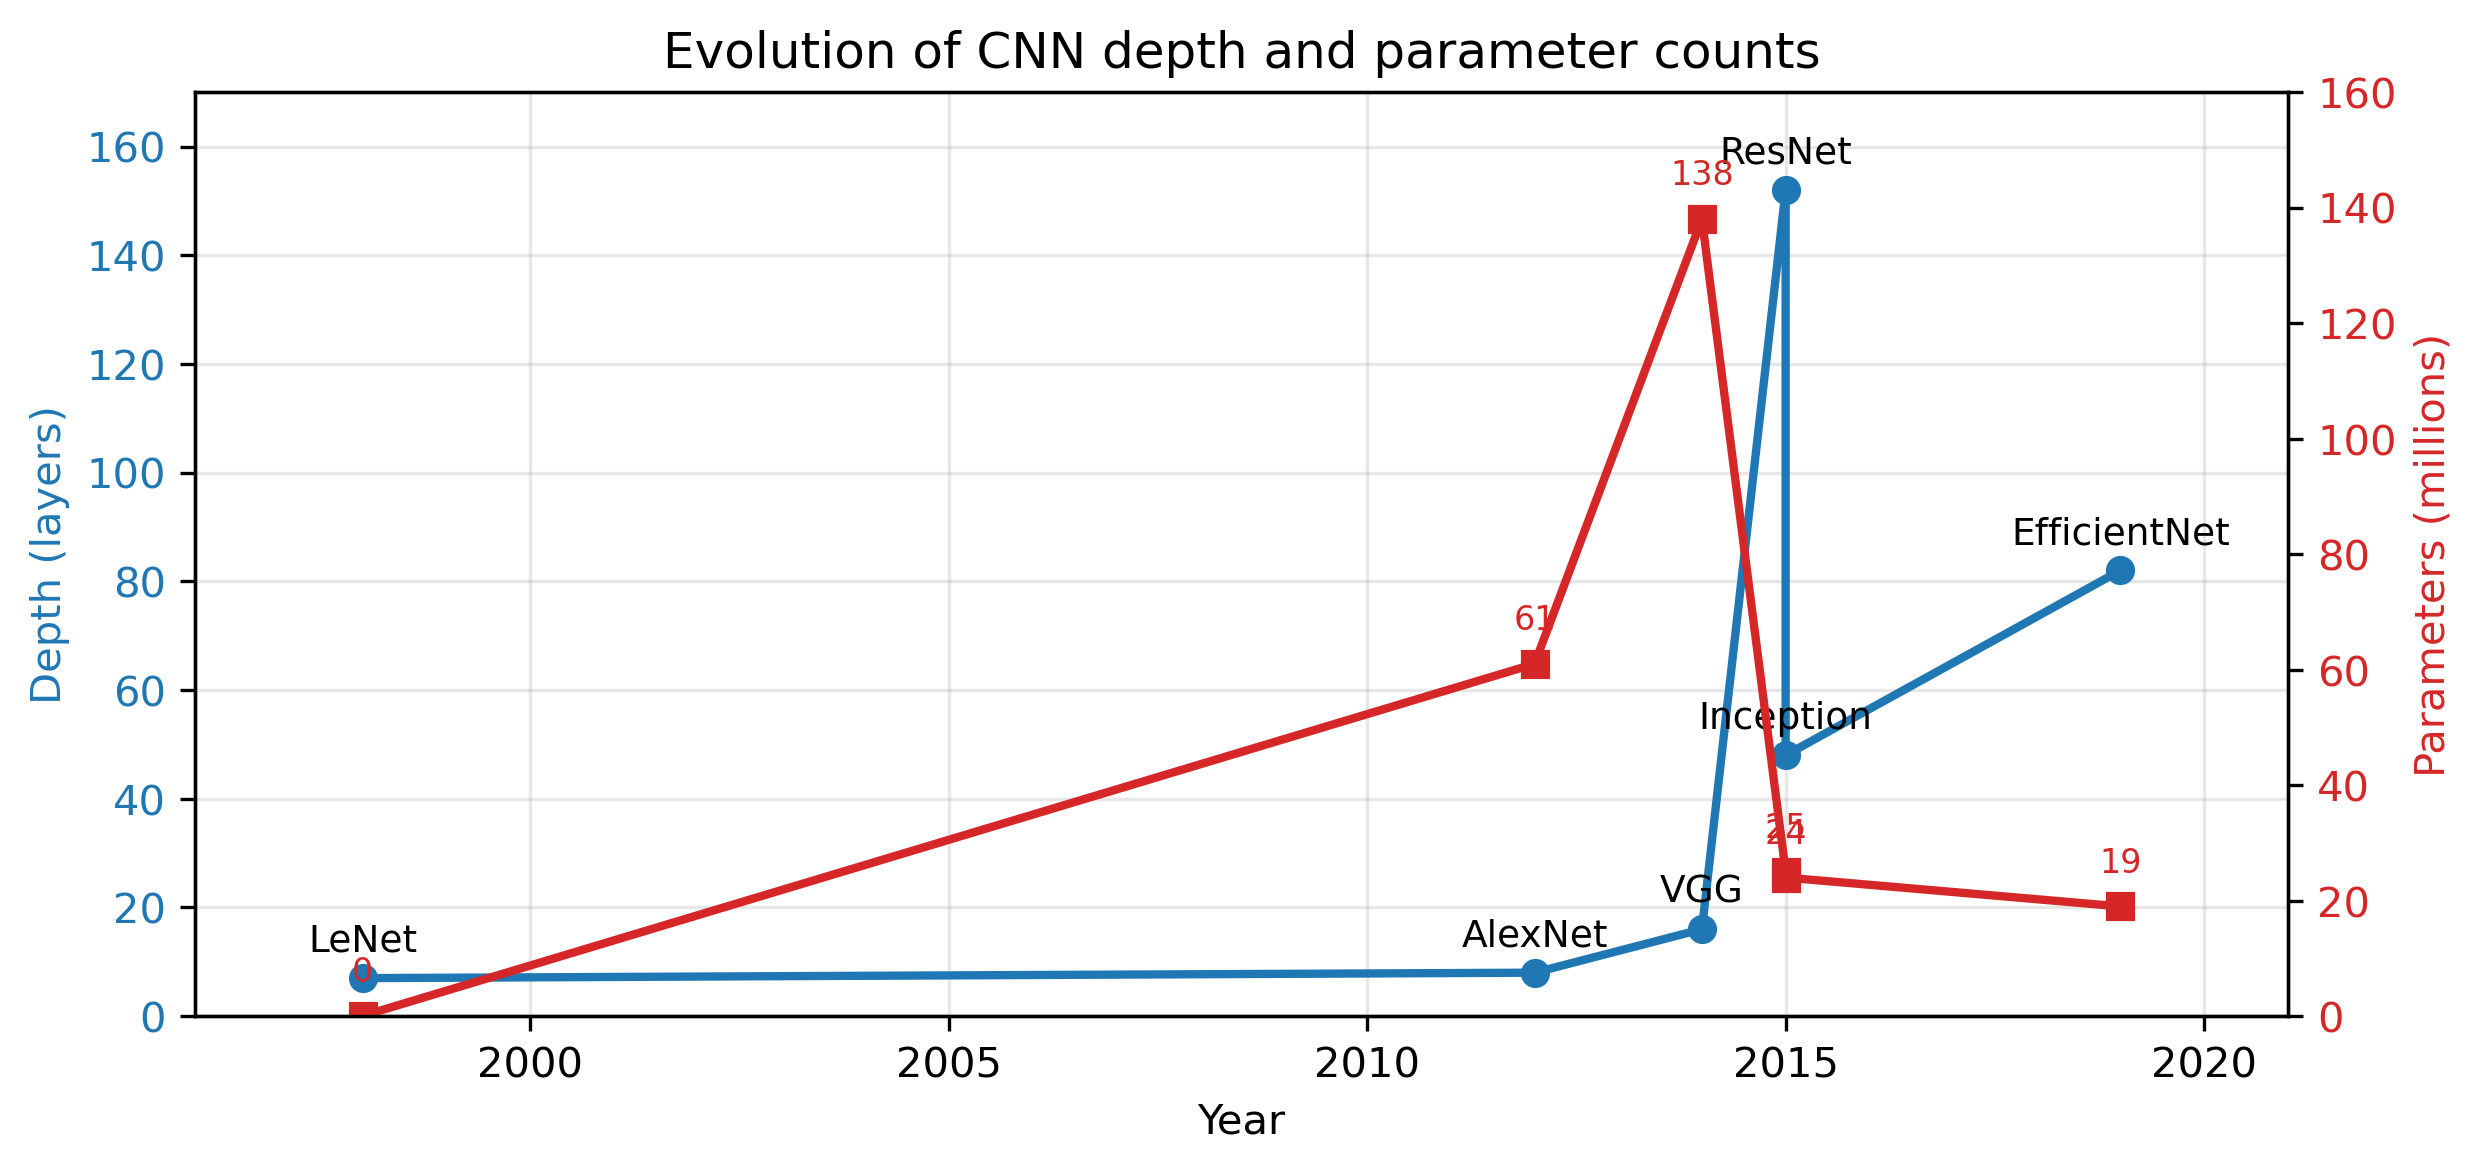
\includegraphics[width=0.85\linewidth]{cnn_architecture_evolution.png}
  \caption{CNN 发展时间线及核心创新。}
  \label{fig:cnn_timeline_cn}
\end{figure}
\FloatBarrier

\section{应用:分类、检测、语义分割等}
CNN 是计算机视觉领域的核心模型,支撑从分类到多模态任务的广泛应用。图~\ref{fig:cnn_applications_cn} 示意了主要任务流程。

\subsection{图像分类}
分类任务通常以 CNN 主干结合全局池化与全连接层输出类别概率。迁移学习通过微调预训练权重提升小数据集表现,Mixup、CutMix 等增强手段能有效抑制过拟合。

\subsection{目标检测}
检测在分类基础上预测物体位置。两阶段检测器(Faster R-CNN)先生成候选框再精炼;单阶段检测器(YOLO、RetinaNet)直接在特征图上回归框与类别。特征金字塔网络充分利用多尺度特征应对大尺寸差异。

\subsection{语义分割}
语义分割为每个像素赋予语义类别。编码器-解码器结构(U-Net、SegNet)通过跳跃连接恢复空间细节;DeepLab 采用空洞卷积与金字塔池化获取多尺度上下文。性能通常用 mIoU 衡量。

\subsection{拓展领域}
CNN 也被用于视频分析(3D 卷积、时空注意力)、医学影像(多尺度 U-Net)、跨模态感知(与 Transformer 融合)。轻量网络如 MobileNet、ShuffleNet 适用于移动端部署。

\begin{figure}[H]
  \centering
  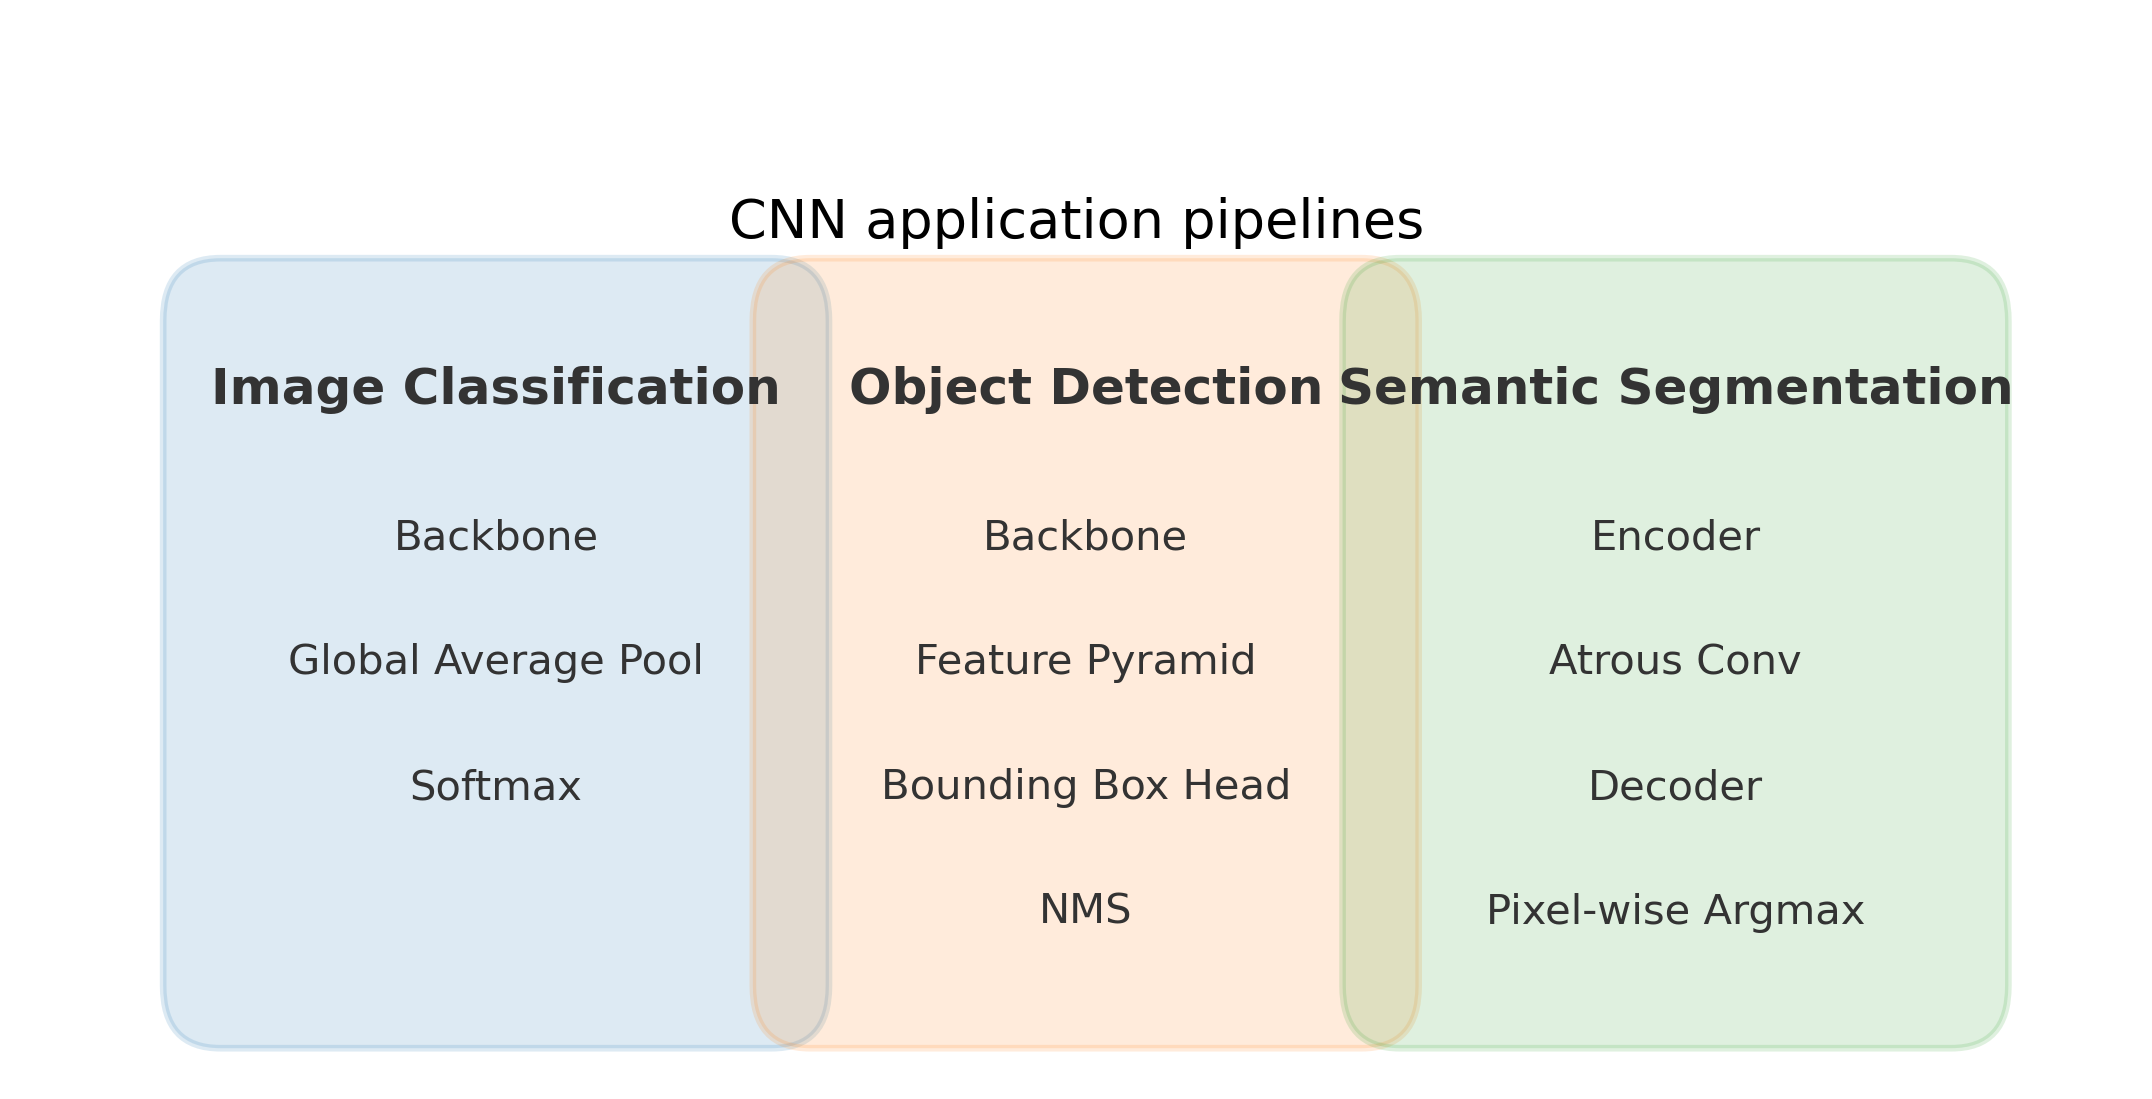
\includegraphics[width=0.85\linewidth]{cnn_applications_overview.png}
  \caption{CNN 在分类、检测、语义分割中的典型流程示意。}
  \label{fig:cnn_applications_cn}
\end{figure}
\FloatBarrier

\section{实践建议}
\begin{itemize}
  \item \textbf{初始化与归一化:} 结合 He 初始化与 BatchNorm/GroupNorm 稳定梯度。\item \textbf{正则化:} 数据增强、dropout、随机深度等策略可提升泛化能力。\item \textbf{优化策略:} 余弦退火 + warmup 的动量 SGD 是稳健基线,自适应优化器适合快速迭代。\item \textbf{效率优化:} 通过深度可分离卷积、剪枝、量化可压缩模型。\item \textbf{指标监控:} 根据任务关注 Top-1 准确率、mAP、mIoU,并可可视化特征图排查问题。\end{itemize}

\end{document}
